\section{Modèle d'exécution fluxionnel}

\subsection{Fluxions}

Le principe du modèle d'exécution fluxionnel est d'identifier des unités d'exécution autonomes n'ayant pour paramètre d'entrée et de sortie que des flux.

Nous avons appelé cette unité d'exécution autonome une fluxion.
C'est à dire une fonction, au sens de la programmation fonctionnelle, dépendant exclusivement de flux de données.
Une fluxion est composé d'un nom unique, d'une fonction de traitement, et d'un contexte d'exécution pour la fonction de traitement.

Les entrée et sortie d'une fluxion sont des flux.
Un flux est un ensemble de message à destination d'une fluxion.
Ces messages sont composé du nom de la fluxion destinataire et optionnellement d'un corps.
Un message peut donc représenter à la fois le signal d'invocation d'une fluxion, et les données nécessaire à son invocation.

À la réception d'un message, la fonction de traitement est invoqué dans son contexte d'exécution, avec le message comme paramètre.
Après avoir traité ce message, la fonction de traitement renvoie un ou plusieurs messages sur le flux de sortie.
La fonction de traitement sait à quelles fluxions les messages de sortie doivent être délivré.
Toute la logique d'une application fluxionnel se trouve dans les fluxions, il n'est pas masqué par une interface de messagerie et un système de routage.

Les fluxions forment des chaînes de traitement lié par les flux.
À la réception d'un premier message, la fluxion destinataire va envoyer un second message à une autre fluxion, qui elle même va renvoyer un troisième message à une fluxion différente, et ainsi de suite.

Le contexte d'exécution de la fonction de traitement est l'ensemble des variables de mémoire dont dépend la fluxion pour poursuivre un traitement d'une exécution à l'autre.
En dehors du contexte d'exécution, la fonction de traitement ne peut pas persister de mémoire d'une exécution à l'autre.

\TODO{	
Les données et la logique d'une application étant cloisonné de manière distincte pendant l'exécution, il est possible de mettre à jour une fluxion en la remplaçant dans le système, sans impacter l'exécution de l'application.
}

Une fluxion peut être déplacée dynamiquement d'environnement d'exécution au cours de son activité.
Déplacer une fluxion nécessite de déplacer sa fonction de traitement ainsi que son contexte d'exécution.
Dans notre approche, nous avons distingué et cloisonné le contexte d'exécution, les paramètres d'appel et les paramètres de retour dans des flux.
Mesurer le débit de ces flux permet d'estimer le coup de leurs déplacements.
Ainsi, déplacer une fluxion consiste à déplacer le code fonctionnel vers une nouvelle destination, puis à rediriger ses flux d'entrées, de sorties et son contexte d'exécution en conséquence.

\subsection{Interface de programmation}

Pour exécuter un programme exprimé sous la forme de fluxions, le modèle d'exécution fluxionnel propose deux fonctions d'interface.

\subsubsection{Enregistrement}

Lors de l'initialisation du programme, il est nécessaire d'enregistrer les fluxions pour qu'elle puisse ensuite recevoir des message.

L'enregistrement se fait à l'aide de la fonction \texttt{register(<nom>, <fn>, <contexte>)}

Le nom de la fluxion lui permet d'être identifié de manière unique dans le modèle d'exécution, et ainsi de recevoir des messages.
Il ne peut donc pas exister plusieurs fluxions ayant le même nom.

La fonction de traitement ne sera appelé qu'avec un seul paramètre : le message reçu.
Ce message peut être vide, auquel cas, ce paramètre sera indéfini.

La fonction de traitement doit renvoyer un message, ou un tableau de plusieurs messages.
Un message se compose du nom de la fluxion destinataire, et optionnellement d'un corps.
Il se construit sous la forme suivante :

\begin{code}
{
  dest: "ma_fluxion", // nom de la fluxion destinataire du message
  body: // corps du message, optionnel
      {}, [], "", ...
}
\end{code}

Une fluxion peut elle-même enregistrer d'autres fluxions dynamiquement.

\subsubsection{Exécution}

L'exécution d'une fluxions n'est déclenché que par la réception d'un message.
L'exécution des fluxions enregistré dans le modèle d'exécution se fait en envoyant un message à une première fluxion.

Ce premier message est envoyé en utilisant la fonction \texttt{start(<nom>,<msg>)}.



\subsection{Système de messagerie}

Le modèle d'exécution fluxionnel repose sur un système de messagerie permettant d'acheminer les flux entre les fluxion selon leurs noms.
Toute l'exécution est orchestré par ce système de messagerie.

Lorsqu'un message ou un groupe de message est soumis à l'envoie, soit par l'appel à \texttt{start}, soit au retour d'une fluxion, le système de messagerie le prend en charge.

Pour chaque message, le système de messagerie vérifie que la fluxion destinataire existe.
Il appel la fonction de traitement de la fluxion destinataire, en utilisant son contexte d'exécution, et avec pour paramètre le corps du message.
La fonction de traitement retourne un message, à son tour soumis à l'envoie.

Les messages soumis à l'envoie sont poussé sur une file de messages, en attendant d'être traité par le système de messagerie.

\subsubsection{Algorithme d'envoi d'un message}

L'implémentation du modèle d'exécution est faites en Javascript.
La file de message est implémenté en utilisant la file d'événements de Node.JS ou du DOM.
La fonction \texttt{postMsg} empile un message dans cette file d'événements en utilisant \texttt{SetTimeout}.

\begin{code}
	// Pousse le message dans la file.
  function postMsg(msg) {
    setTimeout(post, 0, msg);
  }

  // Pour chaque message, on execute la fonction de traitement de la fluxion destinataire.
  function recvMsg(msg) {
    if (!flx_inst[msg.dest]) {
      link(msg.dest);
    }

		// La fonction de traitement de la fluxion destinataire (run) est execute dans son contexte d'execution (scps), avec pour argument le corps du message (body), 
    var res = flx_inst[msg.dest].run.call(flx_inst[msg.dest].scps, msg.body);

    if (res) {
      postMsg(res);
    }
  }

  if (msg)
    if (Array.isArray(msg)) for (var i = 0; i < msg.length; i++) {
      recvMsg(msg[i]);
    } else {
      recvMsg(msg);
    }
\end{code}


\subsection{Interface extérieur}

Le système fluxionnel ne manipule que des fluxion par l'intermédiaire d'un système de messagerie.
Afin de pouvoir interagir avec le monde extérieur, il faut définir des interfaces de bordure.
Les bordures du systèmes sont des fluxions qui font l'interface avec l'extérieur du système.

Notre approche repose sur une espérance de gain technologique principalement sur les architectures Web.
Le premier point d'entré visé est l'intégration des interfaces REST, mais tout autre point d'entrée est valable tant qu'une interface de bordure peut être défini.

Dans notre approche, il existe deux types de fluxion en bordures :

\begin{itemize}
	\item[les \textbf{entrées}]
    permettent de recevoir des connections client entrantes suivant le protocole HTTP.
    C'est donc le premier maillon de la chaîne de traitement.
    Pour chaque connexion entrante, l'entrée va générer une bordure de sortie permettant de répondre au client.
	\item[les \textbf{sorties}]
    permettent d'envoyer le résultat de la chaîne de traitement au client.
    C'est donc le dernier maillon de la chaîne de traitement.
\end{itemize}


Le schéma~\ref{fig:schemaweb} présente les éléments d'un système Web fluxionnel.

\begin{figure}[h!]
	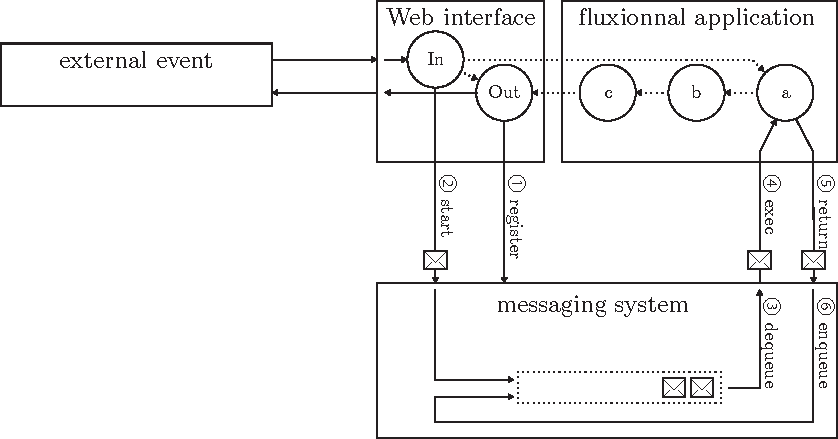
\includegraphics[width=0.5\textwidth]{schema-web.pdf}
	\caption{Schema d'un système fluxionnel avec une interface web}
	\label{fig:schemaweb}
\end{figure}

Le système Web est donc le déclencheur d'une chaîne de traitement de requêtes à chaque nouvelle requête d'un utilisateur un appel à la fonction \lstinline|start('/', <param>)| est réalisé dans le système de messagerie.
Au démarrage du système Web, deux fluxions de bordure sont lancées.
La fluxion de bordure 'in' n'est pas enregistré dans le système de messagerie.
Elle prend les paramètres de la requête Web, place l'identifiant de la connexion client dans le contexte de la demi-fluxion de sortie, puis lance le traitement de la requête en invoquant la fonction `start` du système de messagerie.








